\documentclass[twoside]{uva-inf-bachelor-thesis}
%\usepackage[dutch]{babel}

% Filling your thesis with only lorem ipsum is not advised.
\usepackage{lipsum}
\usepackage{listings}
\usepackage{algorithm}
\usepackage{algpseudocode}
\usepackage{fancyvrb}
\usepackage{xcolor}
\usepackage{subcaption}
\usepackage{graphicx}
\usepackage{commath}

% Citations
\usepackage[style=numeric]{biblatex}
\usepackage[switch, modulo]{lineno}
\linenumbers
\addbibresource{references.bib}

% Title Page
\title{AI-Driven Retrieval and Analysis of Videotaped Council Meeting Archives using Automatic Speech Recognition, Speaker Identification, and Retrieval Augmented Generation}
\author{Pepijn van Wijk}
\supervisors{Dr. Maarten Marx}
\signedby{Signees}

\begin{document}
\maketitle

\begin{abstract}
The accessibility of governmental discussion meetings is fundamental to a healthy democracy, yet current methods for retrieving information from video archives, particularly those of democratically elected councils, are inefficient and time-consuming. This research addresses this issue by leveraging AI to enhance information retrievability from large video archives. By employing state-of-the-art video and audio analysis tools, including a custom Whisper ASR and pyannote.audio speaker diarisation pipeline, videos are transcribed, diarised, and embedded into a Weaviate vector database. 
Archived meetings can subsequently be queried in three different ways: a semantic-based approach utilizing nearest-vector search, a lexical approach employing BM25 ranked keyword search, and a hybrid approach that permits a custom weighted combination of both semantic and lexical search techniques.
These tools significantly improve searchability, as evidenced by the developed system's quicker retrieval times. On top of this, the integration of a chat bot system with access to the Weaviate database offers a conversational interface for querying specific meetings. Overall, this research contributes to enhancing transparency and accessibility in governmental proceedings through AI-driven advancements in information retrieval from video archives.
\end{abstract}

\tableofcontents

\chapter{Introduction}
One of the foundations of a strong democracy is transparency. Citizens must have the opportunity to be informed about- and control the inner workings and decision making process of their (local) governments. To help improve government transparency, Dutch lawmakers introduced the 'Wet Open Overheid' (Woo) \footnote{https://wetten.overheid.nl/BWBR0045754} in 2022. 
This law is applicable to all governmental bodies, from the house of representatives to local municipalities to the tax authority. The three most important terms the Woo brings are: \textit{active publication}, stating government bodies should actively publish some types of information. \textit{Publication on request} states that information should be made public on request. Lastly, the \textit{information management obligation} states that all this information should be easily accessible. 

Various online tools such as the official Woo-index \footnote{https://organisaties.overheid.nl/woo} and Woogle \footnote{https://woogle.wooverheid.nl} offer the ability to search through a wide range of uploaded documents and information. 
Though millions of documents are already published and searchable, the searchability of one important type of information is lacking; the meetings. Decisions, from large to small, are made during long meetings which are livestreamed and archived. These video archives, often three to four hours long, not only require vast amounts of storage, they are also difficult to comb through. For large institutions, manually transcribing meetings and hosting a naive search engine might not be a problem. For the hundreds of small local municipalities however, this is just not feasible in terms of costs and required manpower.

Imagine a journalist writing an article about a new piece of legislation that was, among other things, debated the night before by the local municipality. They want to write what the different parties think of the bill and how they voted. Currently, they would have to watch or skip through to video until they find the part where they talk about the proposed law. Then, they would have to watch the debate and take notes on what each Representative argued, along with their arguments.  Understandably, this simple sounding process quickly becomes both time consuming and inefficient. 
\\ \\
This research provides a solution to this issue by answering the question \textit{how can AI be utilized in order to increase information retrievability of large video archives, in particular of democratically elected councils}? In order to land at a satisfying answer to this research question, some related questions need to be answered first. 
First, the video archives need to be obtained. This means that the first part of this research will be finding an answer to the question \textit{what are the different archive formats local authorities host in order to comply with the Woo and how are these formats exploited to retrieve as much information as possible}?
To extract as much relevant information from the video archives, the question \textit{what state-of-the-art video- and audio analysis tools can be used to improve searchability of the meetings, and how accurate are these in the given circumstances}? needs to be answered. During the aforementioned hour long meetings, many different subjects are discussed. By answering the question \textit{how accurately can such a video be segmented into the meaningfully different parts which are discussed}?, this fact can be used to provide a better overview of the video, as well as enhancing searchability. Finally, an answer to the question \textit{what state-of-the-art information retrieval techniques can be leveraged to develop an efficient video information retrieval system}? should be found, tying everything together.
On top of these base questions, the last part of this research regards an integration of the search system with a large language model, answering the final sub question \textit{how well can the developed search system be integrated with a large language model, creating a helpful chat bot capable of answering questions and providing complementary information when needed}? Building such a chat bot allows for an even quicker answer to questions, without the need to even search for the answer yourself.
\\\\
In summary, the research questions this thesis aims to answer are:
\begin{enumerate}
    \item What are the different archive formats local authorities host in order to comply with the Woo and how are these formats exploited to retrieve as much information as possible?
    \item What state-of-the-art video- and audio analysis tools can be used to improve searchability of the meetings, and how accurate are these in the given circumstances?
    \item How accurately can such a video be segmented into the meaningfully different parts which are discussed?
    \item What state-of-the-art information retrieval techniques can be leveraged to develop an efficient video information retrieval system?
    \item How well can the developed search system be integrated with a large language model, creating a helpful chat bot capable of answering questions and providing complementary information when needed?
    \\
    
    Together, these sub-research questions can be used to answer the main research question:
    \item How can AI be utilized in order to increase information retrievability of large video archives, in particular of democratically elected councils?
\end{enumerate}


\chapter{Related work}
The practice of archiving and transcribing parliamentary meetings is nothing new. Major governmental organisations such as the European Parliament \footnote{https://www.europarl.europa.eu/plenary/nl/debates-video.html} and the Dutch House of Representatives \footnote{https://debatdirect.tweedekamer.nl/} maintain an online archive with basic search functionalities. 
These archives typically provide an engaging user experience by displaying the current speaker and their spoken content. However, the identification of the active speaker often relies on the microphone in use and its assignee, which can lead to inaccuracies when the speaker uses a different microphone than assigned.
Despite the presence of these archives, the search capabilities are often rudimentary, limited to basic keyword searches akin to a simple control+f functionality, or in some cases, no search functionality is provided at all.

In December 2021, students at the University of Washington published the Council Data Project (CDP), an open source municipal data collection tool that includes both front-end and back-end components for searching archived meeting transcripts \cite{Brown2021Council}. 
The CDP primarily focuses on extracting data from municipal archives and employs keyword-based probabilistic information retrieval techniques. However, apart from automatic transcription, the CDP does not utilize machine learning to enhance search functionality.

More recently, in 2023, Italian researchers at the University of Rome developed a system leveraging transcription- and speaker diarisation AI models to process video recordings of Italian Parliament meetings \cite{bertillo2023enhancing}.  This work emphasizes the automation of creating indices but does not offer an extensive search system for the processed video content.

Beyond governmental video archives, prior research has explored the searching of video archives of online lectures. The majority of these studies typically employ a combination of transcript generation and optical character recognition (OCR) to obtain relevant search results, exploiting the fact that on-screen text has a higher probability of being relevant to the presently discussed subject \cite{Adcock10, yang14}. 
However, this approach is not applicable to parliamentary meetings, which generally do not feature on-screen informational text that can be exploited. 

In summary, while existing research has individually addressed AI-based information extraction from governmental meeting archives and search tools for transcribed content, an integrated system combining comprehensive meeting processing with AI-driven search capabilities remains missing.

\chapter{Theoretical background}

\section{Natural Language Processing}
Natural Language Processing (NLP) is the field in computer science primarily focusing on enabling computers to understand human language. Naturally, simply having knowledge of different words and their meaning does not suffice for achieving this goal. A true understanding of language can only be obtained by understanding grammatical rules, contextual details and potential informal vernacular differences in texts from different areas.

% Natural language processing is widely used in everyday life. Whenever you see a foreign article on the internet and use the translate feature to translate this text to English for example. Or, blabla bla bla...

Natural language processing has its historical roots roughly halfway of the previous century. During this time, early experiments were performed trying to create computer chat bots and to automatically translate foreign languages. From the 1950's onwards, an approach that is now called 'symbolic NLP' was used. Symbolic NLP is similar to the way humans learn to understand languages: using a set of handcrafted rules, structures, patterns and decision trees, a framework for the understanding and generation of a language is created. The machine then follows this set of rules to determine the desired output \cite{Dale00}. One example of this symbolic NLP approach is the ELIZA computer program, dating back to 1964. ELIZA was developed by Joseph Weizenbaum at MIT. ELIZA analyzes input sentences by applying a set of generated decomposition rules and key word detection \cite{weizenbaum66} \cite{Jurafsky08}. A response is then generated by a rule set focused on mimicking Rogerian psychotherapy responses \cite{Yao23}. 

\begin{figure}[h]
    \begin{verbatim}
    [User]:  Men are all alike.
    [ELIZA]: IN WHAT WAY?
    [User]:  They're always bugging us about something or other. 
    [ELIZA]: CAN YOU THINK OF A SPECIFIC EXAMPLE?
    [User]:  Well, my boyfriend made me come here.
    [ELIZA]: YOUR BOYFRIEND MADE YOU COME HERE?
    [User]:  He says I'm depressed much of the time
    [ELIZA]: I AM SORRY TO HEAR YOU ARE DEPRESSED
    \end{verbatim}
    \caption{A piece of conversation with ELIZA. \cite{weizenbaum66}}
    \label{fig:eliza-conv}
\end{figure}


With the rapid advances of computational power, the lessening of the dominance Noam Chomsky's linguistics theories and the greater digitisation of written texts, the 80's brought in a natural language processing revolution. The old system of rule sets and decision trees was replaced by a new approach using statistics and machine learning. Instead of following a set of rules, statistical NLP focuses on the identification of common patterns found within a given corpus of language \cite{Manning99}. The detection of these patterns is learned from gigantic bodies of text, called a corpus (plural: corpora). The popularization of the internet and various governments' efforts of digitisation greatly facilitated the collection of these corpora. 
Perhaps the best example of an application of statistical NLP is the predecessor of all current state-of-the-art large language models, the n-gram language model. The n-gram language model works by predicting the occurrence of a word, based on the preceding $n-1$ words. The probability of a word $w_n$ occurring at the end of a sequence of words $w_{n-N+1 : n-1}$ is given by equation \ref{mle} \cite{brown92, Manning99}.
\begin{equation} \label{mle}
    P(w_{n} | w_{n-N+1 : n-1}) = \frac{C(w_{n-N+1 : n-1} w_{n})}{C(w_{n-N+1 : n-1})}
\end{equation}
Here, $N$ is the window of text and $C$ is the count of occurrences, as found in the corpus. 

Naturally, large amounts of text need to be processed in order to form an accurate probabilistic model. Despite being first invented in 1948 by mathematician Claude E. Shannon \cite{shannon48}, the lack of computational power to process these large amounts of text prevented the implementation of the n-gram model until much later.


For many years, the n-gram language model was the state-of-the-art algorithm in language processing. Despite this, it had a significant problem: the curse of dimensionality. The curse of dimensionality is the exponential growth of computational resources needed, when dimensionality of discrete variables increases. To illustrate this, let's say one wants to model the joint distribution of $10$ consecutive words in a language with a vocabulary V of size $100,000$. The amount of free parameters here would total $100,000^{10}-1 = 10^{50}-1$ \cite{bengio03}. 
In 2003, Youshua Bengio et al. proposed a new method of predicting the next word given a sequence of preceding words, utilizing a multi-layer perceptron. Instead of raw strings, it makes use of dense vector representations of words, with semantically similar words embedded closer to each other than meaningfully different words. The continuous nature of these word embeddings inherently do not suffer from the dimensionality curse, since probabilities for (unseen) word sequences are based on the learned similarities between similar vectors. These word feature vectors and the parameters of the probability function are learned during the processing of the training corpus \cite{bengio03}. This innovation gave birth to the current most popular approach to natural language processing: neural NLP.

% Iets over dat strings niet gebruikt worden, maar tokens en word- en sentence segmentation en tokenization enzo (?)
\subsection{Word feature vectors}
As briefly described in the previous section, current state-of-the-art NLP techniques works with embeddings of text. Despite being introduced in the early 2000's, this method did was not successful at corpora containing more than a few hundred millions unique words. In 2013, Google introduced Word2vec, alongside a paper proposing several techniques to train and obtain high quality word vectors, with a larger vocabulary and more accurate than before \cite{mikolov13}.


\begin{figure}
    \centering
    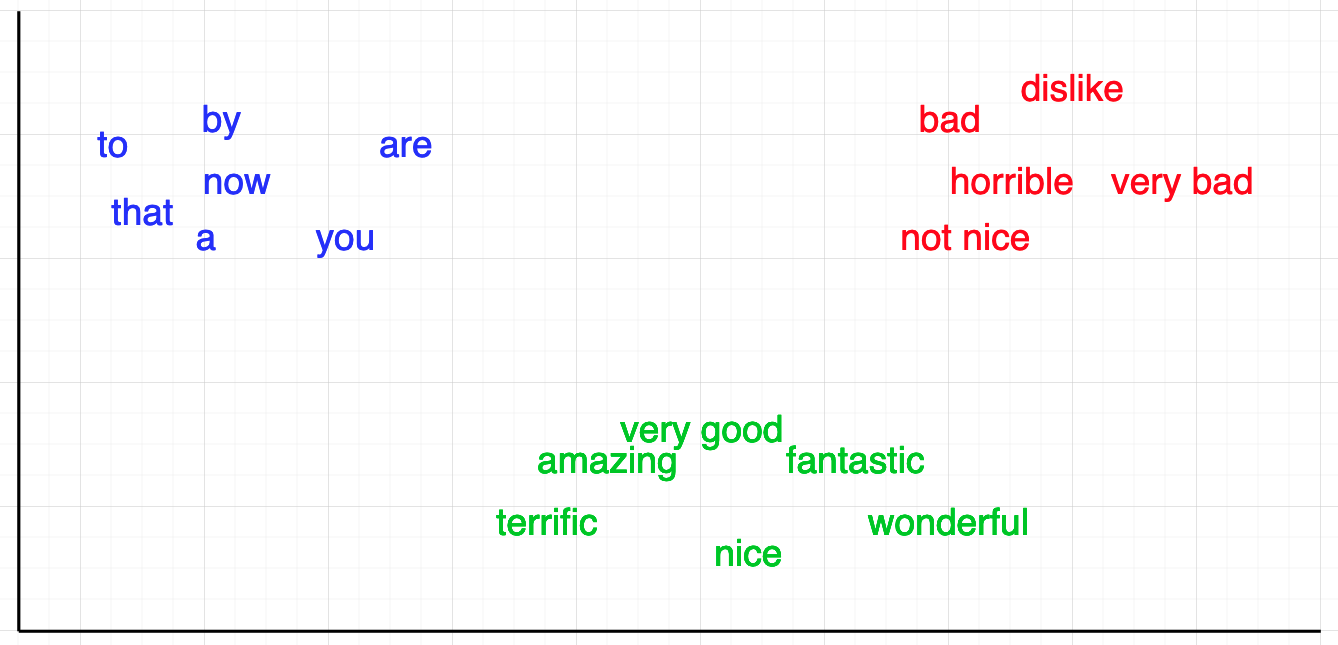
\includegraphics[width=0.85\textwidth]{images/embeddings.png}
    \caption{A two-dimensional (t-SNE) projection of word embeddings. Adapted from \cite{Manning99} and \cite{li16}}
    \label{fig:embeddings}
\end{figure}

remarkably, these vector representations contain an embedded meaning of the word. As stated before, semantically similar words are embedded close to each other in the vector space, a schematic, 2D representation of this phenomenon is illustrated in figure \ref{fig:embeddings}. Besides this locality, word vectors also contain relationships to other words, as learned from the context provided by the dataset. Perhaps the most famous example of this was found by one of the authors of Word2vec, several years earlier \cite{mikolov13_2}. This paper showed that when the vector representing 'Man' ($V('man')$) was deducted from $V('king')$, the result of which added to the vector $V('woman')$, results in a vector closest to the word 'Queen'. Later, the Word2vec paper presented several other examples showing the capabilities of 'word vector arithmetic', as seen in figure \ref{fig:vecarith}.
\begin{figure}[h]
    \centering
    $$V('copper') - V('Cu') + V('zinc') \approx V('Zn')$$
    $$V('Einstein') - V('scientist') + V('Mozart') \approx V('violinist')$$
    $$V('Japan') - V('sushi') + V('Germany') \approx V('bratwurst')$$
    \caption{Word vector arithmetic examples (interpreted as 'zinc is to ... what copper is to Cu'). From \cite{mikolov13}}
    \label{fig:vecarith}
\end{figure}

\subsection{Contextual feature vectors}

Since the end of the 2010's, the implementation of Word2vec is not considered state-of-the-art anymore, being replaced by BERT \cite{devlin19} and GPT \cite{brown20}. The introduction, and consequent improvements of the transformer model shifted the focus in NLP to the utilization of these transformer models. Transformer models are like regular neural networks, but add several so called 'attention layers', allowing words to be processed in relation to all other words in the sequence, taking the specific context into account \cite{vaswani17, vondermosel22}.

\section{Information retrieval} \label{retrievalSection}
According to current Director of the Stanford Artificial Intelligence Laboratory Christopher Manning, information retrieval can be defined as: 

\say{Information Retrieval (IR) is finding material (usually documents) of an unstructured nature (usually text) that satisfies an information need from within large collections (usually stored on computers).}\cite{manning08IR}

This definition steps away from the historic way of searching for data using database systems. In such systems, specific (unique) identifying information such as an order ID or document ID is needed to find data from an information system. Perhaps the most used manifestation that encapsulates this modern way of looking at IR is the Google search engine. The user enters a query, which attempts to communicate the user's information need. The search engine then performs various IR algorithms and ranks results based on their relevance to the entered query. Before the documents can be searched and ranked, they need to be pre-processed. In a process called indexing, a universal representation for the documents is derived that the system can efficiently index.

\begin{figure}[h]
    \centering
    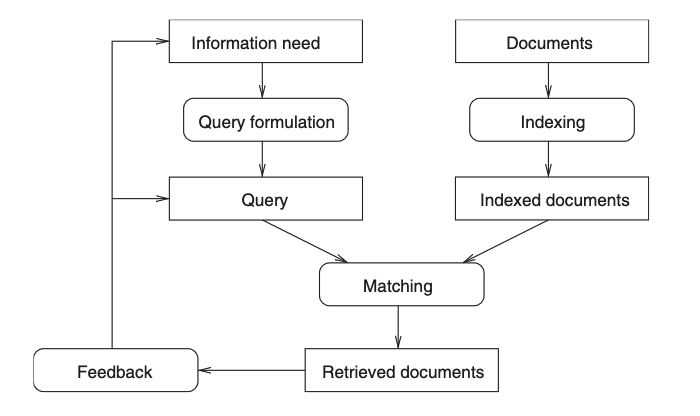
\includegraphics[width=0.85\textwidth]{images/irDiagram.png}
    \caption{Information retrieval process. From \cite{goker2009information}}
    \label{fig:ir}
\end{figure}

Over the years, many different approaches to IR came forward. These different strategies are roughly categorized in three separate models: the boolean model, the probabilistic model and the algebraic model. \cite{goker2009information}

\subsection{Boolean information retrieval}
The boolean model employs a relatively simple and straightforward strategy to information retrieval. A query consists of search terms and potentially the mathematical logical operators AND, OR and NOT. A search term either matches a document, or it does not. Thus, search results can not ranked be ranked like in other models.\cite{goker2009information, manning08IR} An example query that looks for political documents containing the term 'China', but not 'Japan' could look like the following, for example.
\begin{verbatim}
    political AND contains(China) AND NOT contains(Japan)
\end{verbatim}
Due to the fact that boolean queries lack the ability the rank returned results, this model is rarely used in practice. Other models that can rank results and offer the user more freedom to construct searches are favoured in modern systems.

\subsection{Algebraic information retrieval}
The algebraic model facilitates ranked retrieval, in which there is a collection of documents (the corpus), the user issues a query, and a ranked list of documents relevant to the query is returned.

Assume the collection of documents has been pre-processed and indexed into many vectors. Recall that semantically similar words and sentences lie closer in vector space than semantically dissimilar text. Given this fact, similar documents will naturally lie close to each other. Additionally, embedded queries that are relevant to specific documents, will be embedded relatively close to these relevant documents, meaning the measure of similarity between two vectors can function as a ranking score.

The two most popular ranking functions are \textit{Euclidean distance} and \textit{cosine similarity}. Euclidean distance is a widely used metric in clustering problems, measuring the distance between two points in space. Equation \ref{eq:eucDist} gives the general formula for calculating the euclidean distance between two vectors $\textbf{V}$ and $\textbf{W}$ of dimension $n$. \cite{huang2008similarity}
\begin{equation}\label{eq:eucDist}
    D(\textbf{V}, \textbf{W}) = \sqrt{\sum_{i=1}^{n} (V_{i} - W_{i})^{2}}
\end{equation}
Cosine similarity, given in in equation \ref{eq:cossim}, is more popular in textual document information retrieval systems. It is not a metric of distance, but how similar two vector represented documents are. Similarity here, is seen as the angle between two vectors. Thus, unlike Euclidean distance, the difference in magnitude of two vectors has no influence on the metric. \cite{huang2008similarity, rahutomo2012semantic, manning08IR}
\begin{equation}\label{eq:cossim}
    S(\textbf{V}, \textbf{W}) = \frac{\textbf{V} \cdot \textbf{W}}{\lvert \textbf{V} \rvert \times \lvert \textbf{W} \rvert}
\end{equation}

Now, with a means of ranking documents based on a user's query, a search through the corpus is possible. However, the computational complexity to perform a search through all documents scales linearly with the documents. This means that large corpora will quickly become infeasible to query \cite{malkov2018efficient}.

\subsection{Probabilistic information retrieval}
Another model facilitating ranked retrieval is the probabilistic model. Central to this model lies the Probability Ranking Principle (PRP):

\say{If a reference retrieval system’s response to each request is a ranking of the documents in the collection in order of decreasing probability of relevance to the user who submitted the request, where the prob- abilities are estimated as accurately as possible on the basis of what- ever data have been made available to the system for this purpose, the overall effectiveness of the system to its user will be the best that is obtainable on the basis of those data.} \cite{robertson1977probability}

The main challenge of probabilistic information retrieval, is finding a ranking function that efficiently provides an accurate ranking of documents in a collection. 

Central to most probabilistic information retrieval approaches, is the Binary Independence Model. It assumes that a term $q_{i}$ in a document is either present ($1$), or absent ($0$). With this assumption, a search term weight can be computed. While many different weight equations exist, the Inverse Document Frequency (IDF) (equation \ref{eq:idf}) is used most often.
Here, $N$ is the total number of documents, while $n(q_{i})$ is the number of documents containing search term $q_{i}$ \cite{Robertson09}. 

\begin{equation}\label{eq:idf}
    IDF(q_{i}) = \ln{\frac{N - n(q_{i}) + 0.5}{n(q_{i}) +0.5} + 1}
\end{equation}

\subsubsection{Okapi BM25}
Okapi BM25, often referred to simply as BM25, is a high performing ranking function ranking documents based on their relevance to a given search query, dating back to the 70s. It builds upon the Binary Independence Model and incorporates various refinements, allowing for cheap and accurate document scoring.
BM25's ranking function (equation \ref{eq:okapi}) scores each document in a collection for a query by taking into account the frequency of query terms within the document and the document's length \cite{Robertson09, manning08IR}.

\begin{equation}\label{eq:okapi}
    score(D, Q) = \sum^{n}_{i=1} IDF(q_{i}) \cdot \frac{f(q_{i}, D) \cdot (k_{1}+1)}{f(q_{i}, D)+k_{1} \cdot (1-b+b \cdot (\abs{D}/avgdl)}
\end{equation}

Here, $D$ and $Q$ are the document and query containing $q_{1}, ..., q_{n}$ respectfully. $f(q_{i}, D)$ is the frequency of a term $q_{i}$ in document $D$. $\abs{D}$ is the document length, and $avgdl$ is the average document length in the collection. $IDF(q_{i})$ is the inverse document frequency weight of search term $q_{i}$. Lastly, $k_1$ and $b$ are parameters, usually set to $1.2$ and $0.75$ respectfully.

Due to the simplicity and effectiveness BM25 brings, it is still widely used in digital libraries, search engines and other information retrieval systems \cite{Robertson09}.

\subsection{Vector databases}
Vector databases are a relatively new technology that offer a storage and retrieval mechanism optimized for enormous amounts of data, often capable of querying hundreds of millions of documents with only milliseconds latency. 
These remarkable results are achieved by the use of approximate nearest neighbor (ANN) algorithms, offering some accuracy for for a large speed gain \cite{han2023comprehensive}. 

\subsubsection{Hierarchical Navigable Small World graphs}
One of the most employed ANN algorithms is Hierarchical Navigable Small World graphs (HNSW) \cite{malkov2018efficient}. 
This proximity graph based algorithm works on multi-layered graphs, where deeper layers contain more data points and where the deepest layer contains every data point. At query time, the algorithm efficiently navigates these layers to find the approximate nearest neighbors. The process begins at the highest layer, containing fewer data points. In this layer, the closest matching data points are found, after which the nearest neighbors in the layer below are found. This process repeats until the nearest neighbors in the deepest layer have been found. Since there are relatively few data points in the higher layers, many unrelated data points will never be processed, resulting in a quick and efficient search \cite{Malkov2014Approximate}.

\begin{figure}[h]
    \centering
    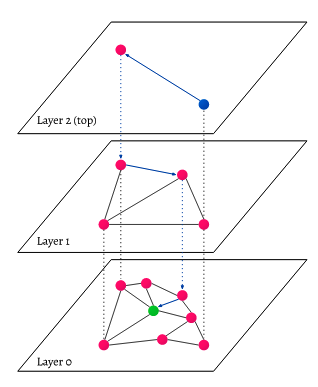
\includegraphics[width=0.4\textwidth]{images/hnsw2.png}
    \caption{A simple Hierarchical Navigable Small World vector search diagram. At each layer, the closest data point is found, resulting in a final best match in the deepest layer.}
    \label{fig:hnsw}
\end{figure}

\subsubsection{Hybrid search}
Generally speaking, dense vector search specialises in the semantic meaning of the search terms, while a keyword search such as BM25 focuses on the search terms themselves and their relative frequency. Many vector databases allow for a combination between such vector similarity searches and probabilistic searches, resulting in a hybrid search taking in to account both keyword frequency and semantic meaning. 


\section{Video \& audio analysis}
Before any of the aforementioned processing and retrieval can be performed, the video must be analysed and pre-processed. As deduced from the stated research questions, the main analysis and processing that is mandatory is transcription, with the use of automatic speech recognition tools, speaker detection, which is done with speaker diarisation models and topic segmentation with the use of large language models.

\subsection{Automatic Speech Recognition}
Automatic Speech Recognition (ASR), informally known as Speech To Text (STT), is the act of transforming spoken language into written text by a computer. ASR has been an old problem, going through many different stages and bringing many technical innovations over the years. 
In the last two decades, the technical advances in ASR led to many consumer products used daily by tens of millions of people such as Amazon's Alexa and Google's home speakers.

One of the very first systems systems capable of recognizing speech was developed in the early 1950's by a research group at Bell Labs. The system was capable of recognizing ten different words: the numbers one through nine - and zero ('oh'). By measuring the spectral peaks resulting from the resonance of the human vocal tract during vowel sounds, known as formant frequencies (figure \ref{fig:ff}), for each digit, the known words could be recognized with an accuracy of 97\% to 99\%. One limitation was that these accuracies could only be reached after preliminary analysis of the speaker's voice. \cite{davis1952automatic, Juang05}

\begin{figure}[h]
    \centering
    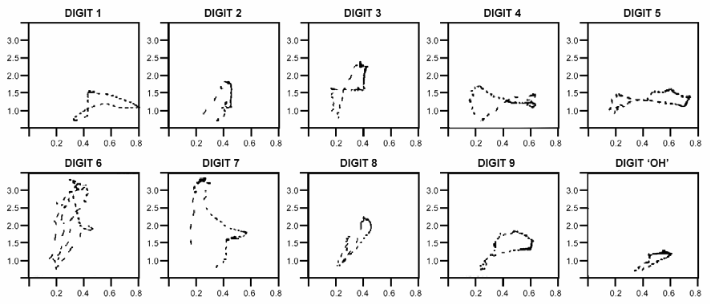
\includegraphics[width=0.9\textwidth]{images/formantFrequencies.png}
    \caption{Photographs of formant frequency presentations of the recognized digits. From \cite{davis1952automatic}}
    \label{fig:ff}
\end{figure}


From the late seventies onwards, a focus on statistical approaches gained traction in favor of the previously used pattern recognition methods. With the use of recently formulated Markov chains and hidden Markov models, subsequent systems rapidly grew to a vocabulary of a thousand word, which was later broken by IBM's Tangora system, capable of recognizing over 20,000 words. \cite{Juang05}

One particularly large milestone was the Sphinx-II system, developed in 1992 by, among others, Xuedong Huang at Carnegie Mellon University. Sphinx-II, using an advanced statistical approach, was the first system that had both a large vocabulary, and the ability to perform speaker-independent detection. The Sphinx-II also won DARPA's speech benchmark evaluation in 1992. ASR systems are mainly evaluated by their Word Error Rate (WER) (equation \ref{eq:wer}) \cite{huang1993overview, huang2014historical}.

\begin{equation} \label{eq:wer}
    WER = \frac{S + D + I}{N}
\end{equation}
where: \\
\begin{conditions}
 S     &  the number of substitutions \\
 D     &  the number of deletions \\   
 I     &  the number of insertions \\
 N     &  the total number of words
\end{conditions}

Up until the late 2000's, the use of hidden Markov models and similar statistical methods still dominated in the ASR space. However, with the advent of deep neural networks (DNNs) and the aforementioned transformer architecture, the paradigm has shifted yet again, bringing light the the current state-of-the-art: OpenAI's Whisper ASR.

\subsubsection{Whisper}\label{sec:whisper}
In 2022, OpenAI released Whisper, capable of 'Robust Speech Recognition via Large-Scale Weak Supervision' \cite{radford2023robust}. Trained on 563,000 hours of labeled English speech, and 117,000 hours of labeled speech in 96 different languages, Whisper is the current state-of-the-art ASR system, with a (post normalisation) word error rate that is similar to a professional human transcriber, as seen in figure \ref{fig:whisperwer}.
Whisper makes use of an encode-decoder Transformer, as described in \cite{vaswani17}. Input audio is first resampled and standardized, after which it is converted to a Mel Spectrogram, normalized and fed in to the network. A full view of the simplified architecture can be seen in figure \ref{fig:whisperarch}.

\begin{figure}
    \centering
    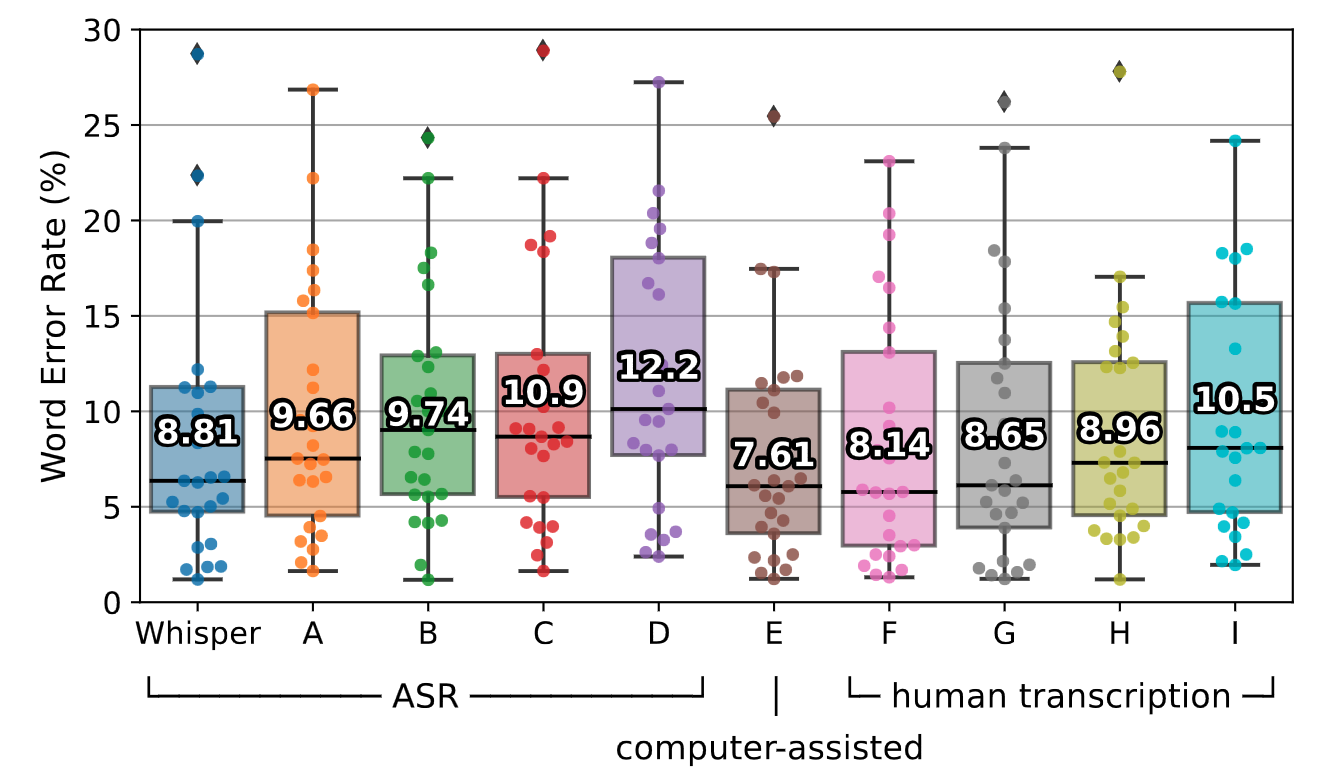
\includegraphics[width=0.8\textwidth]{images/whisperwer.png}
    \caption{Whisper WER compared to other companies and human professionals. From \cite{radford2023robust}}
    \label{fig:whisperwer}
\end{figure}

\begin{figure}
    \centering
    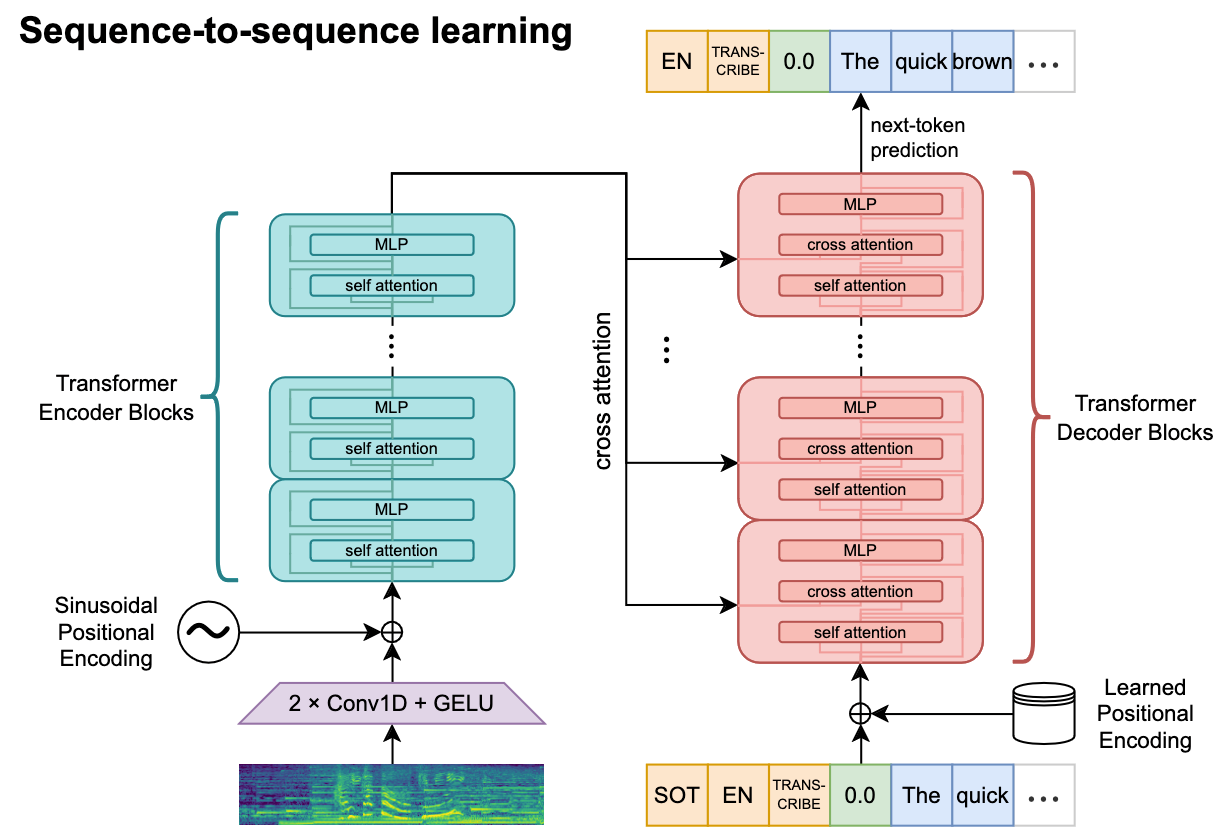
\includegraphics[width=0.9\textwidth]{images/whisperarch.png}
    \caption{Simplified Whisper architecture. From \cite{radford2023robust}}
    \label{fig:whisperarch}
\end{figure}

\subsection{Speaker diarisation}
Speaker diarisation (SD) is the process of partitioning input audio containing multiple speakers, in to separate segments containing single speakers. It aims to solve the question 'Who spoke when?' \cite{sahidullah2019speed}. Speaker diarisation is a relatively new problem. In film and news studios the central question is not necessarily a mystery; different speakers have different microphones, whose data is known and separate at the time of processing and editing. 

\begin{figure}[h]
    \centering
    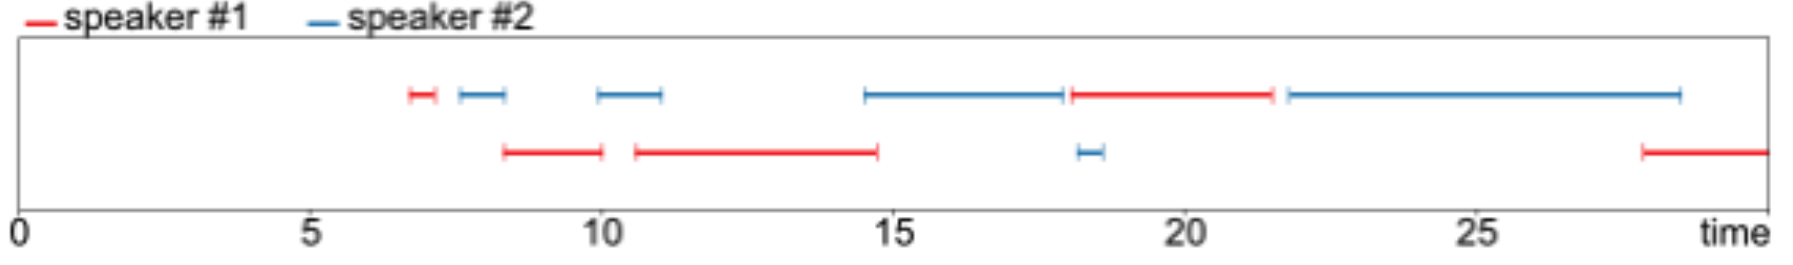
\includegraphics[width=0.75\textwidth]{images/speakerdiaroutput2.png}
    \caption{Desired speaker diarisation result. From \cite{bredin2023pyannote}}
    \label{fig:sdo}
\end{figure}

Central to speaker diarisation is voice profile feature extraction. When a reliable and accurate method of embedding voice profiles is achieved, these voice profile vectors can be compared using similarity measures such as cosine similarity or euclidean distance to find different speakers and when they speak. Different systems utilize different methods of obtaining feature vectors. Most of these feature extractors use various representations of sound waves, with additional features derived from pitch information and audio metadata, mostly from the standardised MPEG-7 audio standard \cite{kotti2008speaker, lu2002speaker}. Some of the most common features have a similar accuracy, Mel-frequency cepstral coefficients
(MFCCs) \cite{gook04} and Line spectral pairs (LSPs) \cite{lu2002speaker}. 

\subsubsection{Pyannote}\label{sec:pyannote}
 Pyannote.audio (pyannote) is the current state-of-the-art speaker diarisation mode. It is not only a speaker diarisation model, but it also offers a range of speaker diarisation sub-modules. These submodules include voice activity detection, overlapped detection speech, speaker change detection, and more. \cite{bredin2020pyannote, bredin2023pyannote}

In most competitions, speaker diarisation accuracy is graded by four criteria: speaker confusion rate (CONF), which is the duration of speaking where the speaker is mislabeled, false alarm rate (FALSE), which is the duration of non-speech incorrectly classified as speech, missed detection (MISS), which is the duration of speech that is incorrectly classified as non-speech and Diarisation Error Rate (DER), which is a combination of the first three. As can be seen from figure \ref{fig:pyanres}, pyannote scores at the top of most benchmarks. Top benchmarks are greatly improved by their preview baseline, while DERs on benchmarks where pyannote does not score at the top are fairly close, indicating a great overall performance. \cite{bredin2023pyannote}

\begin{equation}
    DER = \frac{FALSE + CONF + MISS}{ground \; truth \; duration}
\end{equation}

The pyannote system uses the following distinct steps on five seconds sliding windows of audio \cite{bredin2023pyannote}: 
\begin{enumerate}
    \item Local speaker segmentation, where these windows are analysed for different speakers and when these different speakers start- and stop speaking.
    \item Local speaker embedding, where the voice profiles of the different speakers in the sliding windows get embedded.
    \item Global agglomerative clustering, where local speakers are grouped into global clusters. 
\end{enumerate}

Pyannote diarisation outputs are formatted according to the Rich Transcription Time Marked (RTTM) file format, described in \cite{ryant2018first}.

\begin{figure}
    \centering
    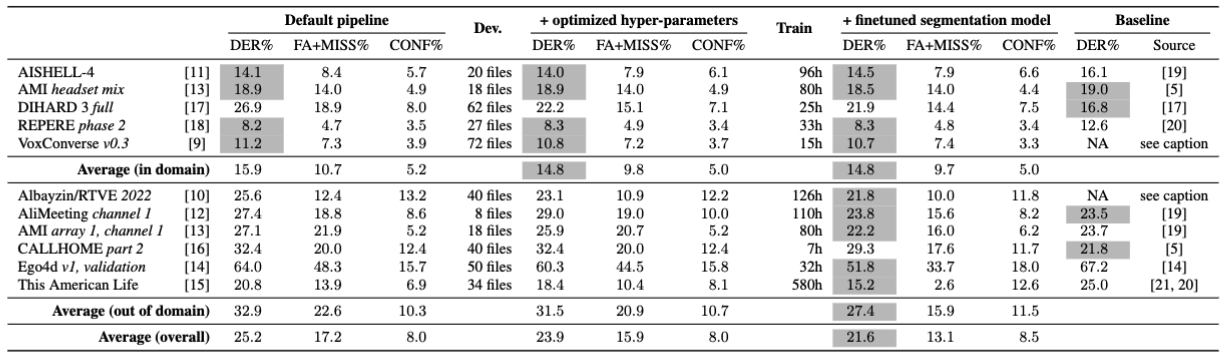
\includegraphics[width=0.99\textwidth]{images/pyanresults2.png}
    \caption{Performance of the (default, optimized, and fine-tuned) pipelines on 11 different benchmarks. The grey background marks the best results for each dataset as well as those less than 5\% worse relatively. From \cite{bredin2023pyannote}}
    \label{fig:pyanres}
\end{figure}

% \subsection{Topic segmentation}
% \lipsum[4]

\section{Retrieval Augmented Generation}
Large Language Models (LLMs) store vast amounts of factual information within their parameters. For certain knowledge intensive queries or queries that require proprietary information not included in the training data, an LLM's knowledge recalling abilities are not enough. These situations require external information provided in the prompt that the LLM can use to give a complete and accurate answer \cite{NEURIPS2020_6b493230}. Retrieval Augmented Generation (RAG) is the process of enhancing the LLM's question answering capabilities by finding relevant context and documents and providing these to the LLM in the prompt. The LLM will then use the provided information to answer the user's question more accurate and with less hallucinations.

The retrieval of the relevant context is mostly done by the use of a dense vector index or any other retrieval method described in section \ref{retrievalSection}.

\begin{figure}
    \centering
    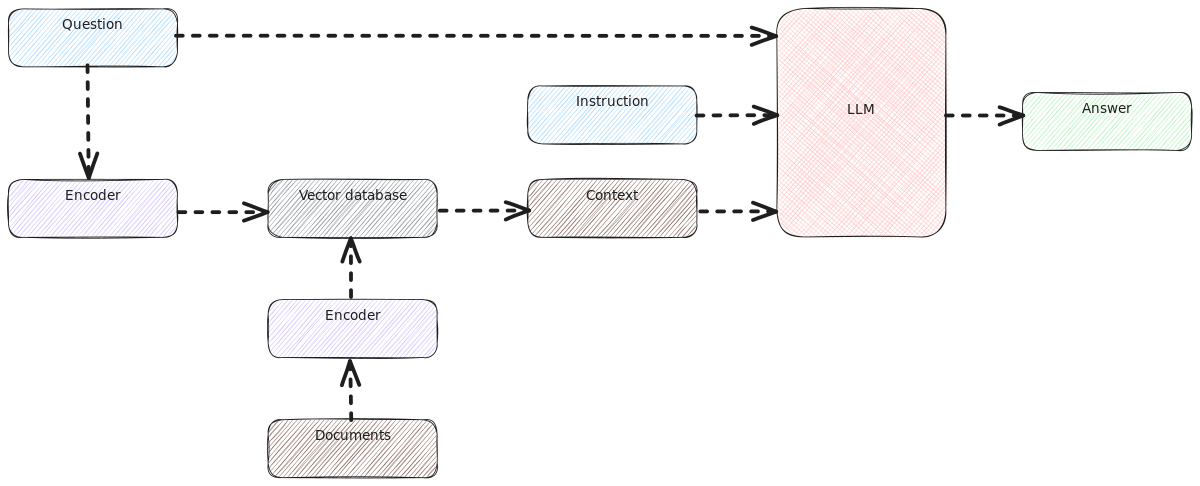
\includegraphics[width=0.9\textwidth]{images/rag.png}
    \caption{Retrieval Augmented Generation pipeline}
    \label{fig:rag}
\end{figure}


\chapter{Methods}
\section{Archival data extraction}
Before starting any analysis work, the first research question, \textit{what are the different archive formats local authorities host in order to comply with the Woo and how are these formats exploited to retrieve as much information as possible?}, needs to be answered.

An overwhelming amount of Dutch municipalities are allied with one of two service providers that archive, host and index past council meetings. These two service providers are \href{https://www.ibabs.com}{iBabs} and \href{https://www.notubiz.nl/}{NotuBiz}. NotuBiz alone serves over 250 local municipalities, provinces and water authorities, while iBabs serves several hundred more. 

Thus, in order to create a service compatible with most Dutch governmental bodies, a tool must be developed that is capable of extracting meetings from at least these two hosting services.

\subsubsection{NotuBiz}
NotuBiz serves many municipalities in an easy to scrape, static format. Municipalities have the option to host meetings of different categories and NotuBiz allows for a search to be performed on many different objects such as meeting points, documents, years and meeting types.
When searching for a specific meeting type, NotuBiz sends a GET request to a remote server. By sniffing the network upon making such a search request, I identified the endpoint used for meeting searches and its necessary parameters. 
The important parameters are \textit{keywords}, meaning the meeting type, and \textit{organisations}. 
This organisations parameter is quite cumbersome, since it is a municipality specific code used to specify the municipality to be searched. The only way to retrieve this is to make a search request on the desired NotuBiz website and to sniff the network. 

I have created a scrape script in a Python Jupyter Notebook that can scrape any NotuBiz archive with minimal user input needed. The user must simply provide the municipality name, the download location, the base NotuBiz URL, the desired meeting types and years and the unique municipality code mentioned earlier. 
The script will then find all meetings using Python's Beautiful Soup library, writing the meeting page links to a file. When all meeting links are found, the webpages are parsed to look for the remote URL where the video is hosted. When this link has been found on the page, the video will be downloaded and saved at the location specified earlier.

\subsubsection{iBabs}
Unlike NotuBiz, iBabs is a dynamically loaded site, meaning data gets loaded in and out of the browser in real-time as users interact with the site. One positive result of this approach is that it enables more responsive and interactive user experiences, as the web page (DOM) can update content without requiring a full page reload. A negative effect is that it makes it more difficult to scrape the webpage for its information and videos with simple scraping tools.
In addition to this fact, iBabs also uses a specific file format for their video archives, M3U. M3U is not a video file, it is a text file that specifies the locations of parts of a video or audio file hosted on a remote server, allowing for more efficient streaming. 
Unlike NotuBiz, where the video link is statically present in the web page, the M3U file on iBabs is only fetched from the server when the user clicks the \textit{play video} button. 

Both these complications mean that static scraping tools and HTML parsers such as Python's urllib and Beautiful Soup are not equipped to deal with iBabs. To solve these issues, I used Selenium Web Driver. Selenium is an automatable web browser that can be programmed to interact with the DOM and parse web pages. Selenium can also be used to sniff the browser's network for the M3U URL that is fetched from the iBabs servers when the \textit{play video} button is clicked. 

Similar to NotuBiz, I have written a generic iBabs Jupyter Notebook scraper. The user only has to specify the municipality name, the download location and which years should be retrieved. 
The tool will then fetch all categories that are listen on the home page using Beautiful Soup, creating directories for the municipality, its categories and for each category the different years in the process.
Next it will use Beautiful Soup to get links to all pages hosting different videos and writes these links URLs to a file containing all meeting webpage URLs. 
When all video pages have been scraped, Selenium is used to open each page, find and click the \textit{play video} button. After this, the browser network is sniffed for the fetched M3U file link which is written to the another file.

After all M3U URLs have been retrieved, the file containing the download links is read and videos are downloaded using a M3U download tool \footnote{https://github.com/josephcappadona/m3u8downloader}.


\section{Video- and audio analysis}
This section explains the design and design choices made in order to answer the second research question, \textit{What state-of-the-art video- and audio analysis tools can be used to improve searchability of the meetings, and how accurate are these in the given circumstances}?

Machine learning is a constantly changing field that evolves rapidly. Every month, dozens of new models and model architectures are released that are more effective in specific niche scenarios. 
With this in mind, one of the fundamental principles I decided to uphold in the creation of the analysis pipeline, is that the design of the AI clients must be as modular as possible. This is primarily achieved through the implementation of Python class inheritance. 

\subsection{Whisper}
The ASR client, responsible for transcribing downloaded meetings, is implemented with Whisper ASR for reasons explained in section \ref{sec:whisper}.
As for the ASR client, A base \textit{Transcriber} class specifying what methods must be implemented is defined. Then, for each new ASR model, a child class can be created where only model-specific methods are written. 
In the case of the ASR client, the only model-specific method that must be implemented is the \textit{transcribe} method. \textit{transcribe} should take in an input path and an output path, which will be used to load the audio file and save the transcription.
Other methods such as loading transcriptions are model invariant.

In the current analysis pipeline code, two transcriber classes have been implemented: one client using Whisper on MLX, a Python array framework allowing fast machine learning on Apple silicon devices, and one using the official Whisper implementation on PyTorch. Since the underlying models and weights are the same however, there will not be a difference in the output of these two different transcribers.

\begin{lstlisting}[language=Python, caption={Modular transcriber class implemented in Apple's MLX Whisper port and PyTorch's Whisper port.}]
class Transcriber:
    def transcribe(self, input_file, output_file):
        print("Transcribe method not implemented!")
        return  WhisperReturnCodes.NOT_IMPLEMENTED

    def load_transcription(self, path):
        # Logic which is not specific to any particular model.
        return transcription


class MLX_Transcriber(Transcriber):
    def __init__(self, model):
        self.model = model

    def transcribe(self, input_file, output_file):
        # MLX whisper transcribe logic.
        return

class Torch_Transcriber(Transcriber):
    def __init__(self):
        self.model = whisper.load_model("medium")

    def transcribe(self, input_file, output_file):
        # PyTorch whisper transcribe logic.
        return
\end{lstlisting}

\subsection{pyannote}
The speaker diarisation client is designed following the same principles and methodologies as those employed in the Whisper client. A base class \textit{Diarisor} defining the model-specific methods is declared, which is used as a parent class by model specific classes, in the case of this project, the \textit{Pyannote} class.

The speaker diarisation client has two model-dependant methods: \textit{diarise} and \textit{embed}. The \textit{diarise} method takes in an input path and an output path, which are used to load the audio and save the generated speaker diarisation output. The \textit{embed} method takes in an input file and a start- and end time. It will then embed the voice profile of the audio within the specified time frame.

As mentioned in section \ref{sec:pyannote}, pyannote.audio is the current state-of-the-art in the field of speaker segmentation. Because of this, the model used in the final architecture is pyannote.audio V3.2.0, the latest version. In case a new, better model is released, this model can be easily implemented due to the modular design of the client.

\begin{lstlisting}[language=Python, caption={Modular speaker diarisation class.}]
class Diarisor:
    def diarise(self, input_file, output_file):
        print("Diarise method not implemented!")
        return PyannoteReturnCodes.NOT_IMPLEMENTED

    def embed(self, input_file, from_time, to_time):
        print("Embed method not implemented!")
        return PyannoteReturnCodes.NOT_IMPLEMENTED
\end{lstlisting}

\subsection{Embedder}
Practically all sentence embedding models present day are released on HuggingFace, making modularisation easy. HuggingFace embed models can be used through a standard method \textit{encode} in the SentenceTransformers framework developed by HuggingFace. This means that only the class initialisation method is model-specific, while the embed method can be model invariant since it is called through the SentenceTransformers API.

\begin{lstlisting}[language=Python, caption={Modular embed class.}]
class Embedder:
    def __init__(self):
        print("Init method not implemented!")
        return EmbedReturnCodes.NOT_IMPLEMENTED

    def embed(self, text):
        if not self.model:
            return EmbedReturnCodes.NO_MODEL

        return self.model.encode(text)
\end{lstlisting}

Choosing the appropriate embedding model for this project is not as simple as looking at the current leaderboard and selecting the top-performing model. The reason for this is the vast array of available embedding models, each optimised for specific niche applications. 
The primary requirements for this project be lightweight, fast, and multilingual. Given that thousands of hours of video material need to be embedded, a model with low computational demands and rapid processing capabilities is crucial. Even more important however, is the requirement for multilinguality. Multilinguality ensures that semantically similar sentences in different languages will still map close to each other in the vector space. Since most monolingual embedding model are trained on English text, running these models on Dutch sentences will lead to suboptimal performance.

In the end I selected the sentence-transformers/all-mpnet-base-v2 model \footnote{https://huggingface.co/sentence-transformers/all-mpnet-base-v2}. Its compact size of only 109 million parameters, coupled with its multilingual capabilities make it the perfect model for this task.

\section{Agenda point segmentation}\label{sec:agendapoints}
To answer research question three, \textit{how accurately can such a video be segmented into the meaningfully different parts which are discussed}, an agenda point topic segmentation client needs to be written. It should take in the transcript of a meeting, and it should return a list of agenda points and times, specifying when these topics start and end.

% As it turned out, some of the meetings already have their agenda points provided by the archiving host. For the meetings where this is not the case, a custom agenda point generator that utilizes LLMs has been written.

The concept of the topic segmentation client is quite simple. First, the transcript of a meeting is fed into an LLM with the task to label the most important topics discussed during the meeting, in chronological order. 
Next, for each topic, the LLM should figure out when the agenda point starts in the meeting. This is done using a sliding window over the transcript. 
One by one, sentences, along with their starting time and the current topic, are sent to a LLM. The LLM is then tasked to return either true or false depending on if it thinks the agenda point starts at the current sentence. When this is the case, the topic is considered labeled and the next topic is prompted. 
A pseudocode representation of this algorithm is presented in \ref{alg:topic}.

\begin{algorithm}
\caption{Agenda topic Segmentation Algorithm}
\label{alg:topic}
\begin{algorithmic}
    \Require Transcript $T$ of a meeting
    \State $Topics \gets LLM(T, \text{task="label"})$
    
    \For{each $Topic$ in $Topics$}
        \State $Timed \gets \text{False}$
        \State $i \gets 1$
        
        \While{not $Timed$ and $i \leq \text{length}(T)$}
            \State $Sentence \gets T[i]$
            \State $Response \gets LLM(\text{input=}\{Sentence, Topic\}, \text{task="topicStart?"})$
            
            \If{$Response$ is True}
                \State $StartTime \gets \text{getStartTime}(Sentence)$
                \State $Timed \gets \text{True}$
            \Else
                \State $i \gets i + 1$
            \EndIf
        \EndWhile
    \EndFor
    
    \State \Return $TimedTopics$
\end{algorithmic}
\end{algorithm}

\section{Information retrieval}\label{sec:weaviate}
For research question four, \textit{What state-of-the-art information retrieval techniques can be leveraged to develop an efficient video information retrieval system}?, a Weaviate vector database Python client has been built.
The created Weaviate client allows the user to easily perform simple operations such as creating and deleting collections (similar to tables in relational databases), inserting and deleting entries and getting collection metadata. 
Besides these basic operations, three search methods described in section \ref{retrievalSection} have been implemented: Vector search, BM25 search and Hybrid search.

All search methods allow the user to specify filter parameters such as government, year, speaker and more. Invariant of employed the search method, the client returns data in a uniform format—an array of relevant result objects. Each result object within this array includes properties such as meeting ID, government, year, etc., the result's UUID, its vector representation, and its relevance score.

The Weaviate database consists of two different collections: \textit{Transcripts} and \textit{Speakers}. The \textit{Transcripts} collection is organised by uninterrupted speaking turns of individuals. Each entry within this collection is linked to the embedding of the content of this speaking turn, as well as to the voice profile embedding of the speaker.
The \textit{Speakers} collection is indexed by voice profile embeddings. This collection associates each voice profile with a corresponding speaker's name, providing the web application the ability to map each speaking turn to the correct speaker's identity.


\section{RAG chat bot}

RAG consists of two parts: retrieval and generation. A user query is first fed in to the retrieval system which returns one or more pieces of context that are most relevant to the specified query. Next, this context is added to the user query after which a LLM will answer the query using the acquired context. 

In essence, the created chat bot pipeline is similar to figure \ref{fig:rag}. The final web app uses a BM25 based retrieval pipeline as specified in section \ref{sec:weaviate}. If no results are found, this is signaled to the user and the process is aborted. In the likely scenario that results are found, the results are added to the query and the LLM is called to answer the question.

Identical to the other clients, the LLM client designed to be modular and easily swapped. The base model only has a single model dependant method: \textit{run}. \textit{run} takes the chat history as an arguments and prompts the LLM. 
In the final product one of two LLM clients are used: A locally running Llama client or a GPT client that calls the OpenAI API. The former can be used on machines that have sufficient RAM and a strong GPU. The latter is recommended for other machines. Since it calls the OpenAI GPT API it is both quick and accurate, bringing with it only a small cost of \$15 per one million output tokens.

\begin{lstlisting}[language=Python, caption={Modular LLM class.}]
class LLM:
    def run(self, history):
        print("run method not implemented!")
        return LLMReturnCodes.NOT_IMPLEMENTED
\end{lstlisting}

\section{Search engine}
To answer the main research question, \textit{How can AI be utilized in order to increase information retrievability of large video archives, in particular of democratically elected councils?}, all previously mentioned functionalities should be combined. To do this, I created a user-friendly search engine using front-end framework Vue3.

The web app offers two primary functionalities. The first is a global search feature, 
enabling users to search through all available videos for spoken information. For more specific queries, users can apply selectable filters to search by a particular government, meeting type, or year.

The second functionality allows users to navigate the video archive by selecting the government, meeting type, and year. Once a video is selected, it is displayed and can be played. 
Below the video, the speakers, their speaking turns, and the meeting discussion points with corresponding timestamps are shown. Clicking on a speaker or discussion point advances the video to the relevant timestamp. Additionally, a search bar beneath the video, similar to the global search, permits users to search within the video for specific information. This in-video search also supports filtering by speakers and discussion points.

Adjacent to the video, a LLM powered chat window enables users to ask questions and retrieve information related to the video content in a conversational way.
\begin{figure}
    \centering
    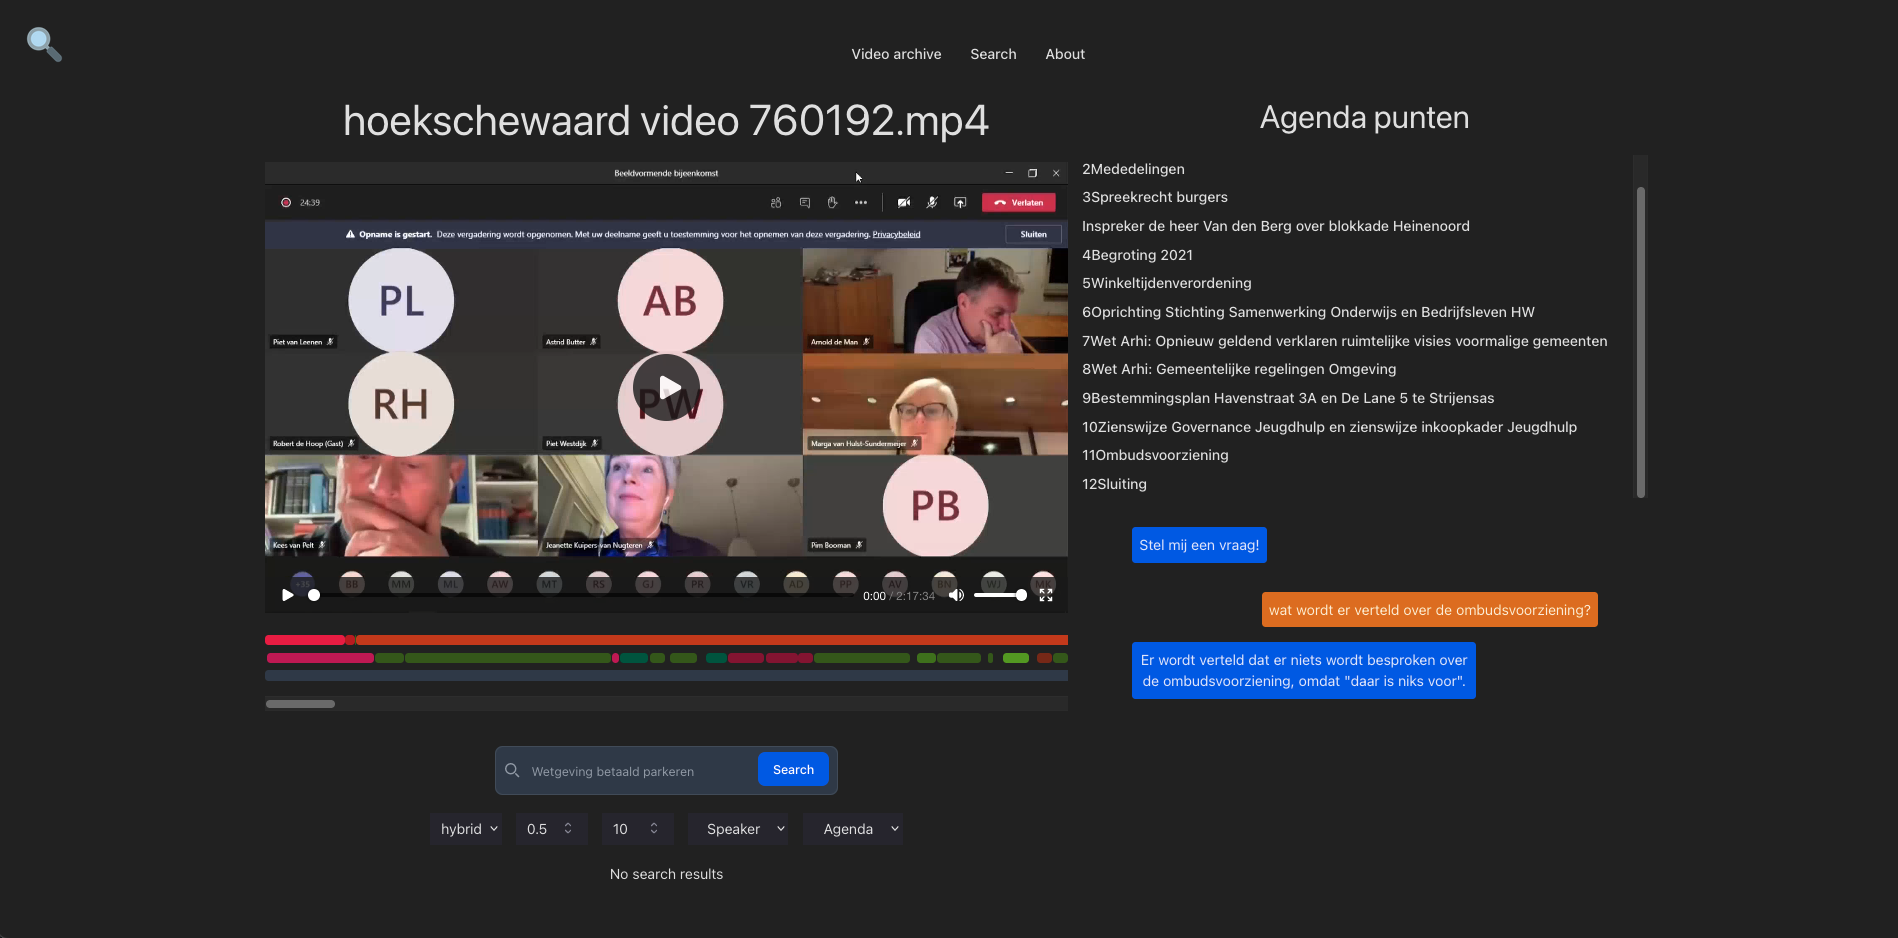
\includegraphics[width=0.9\textwidth]{images/frontend.png}
    \caption{Web application video view}
    \label{fig:frontendVid}
\end{figure}

\subsection{Analysis pipeline}
Before a municipality can be added to the archive, all meetings have to be downloaded and analysed. A diagram of the analysis pipeline is shown in figure \ref{fig:pipeline}.

\begin{figure}
    \centering
    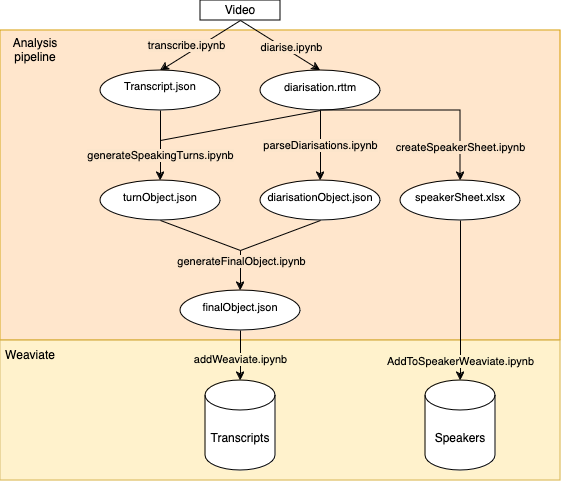
\includegraphics[width=0.85\textwidth]{images/pipeline.png}
    \caption{Video analysis pipeline}
    \label{fig:pipeline}
\end{figure}

The two most important analysis scripts are \textit{transcribe} and \textit{diarise}. These script run Whisper and pyannote respectively, and create a file containing the transcript and diarisation. data. the diarisation data is then used to create a diarisationObject, a JSON file containing the voice profile embedding of each speaker and when they are speaking. Also, a speakerSheet is created. This is and Excel file that an administrator should fill in manually. It maps a detected speaker to a given name, allowing speaker recognition including names. Annotated speakers will also be available for videos that were not annotated, meaning that manual speaker labeling only has to be done a single time per speaker.

The transcript and diarisation information together are used to create a turnObject. This is a JSON file that contains text of each speaking turn for each speaker and the textual embedding. When this file is created it is combined with the diarisationObject in order to create the final objects that will be added to Weaviate.

\subsection{Deployability}
The entire search engine web app, its back-end and the Weaviate vector database are easily deployed using a custom Docker script. In total, over three thousand hours of meetings has been collected and analysed. The raw video files for these meetings alone are over 2 terabytes. Due to this large storage requirement, The docker image does not include the videos, only the extracted information needed by the front-end and Weaviate.
This necessary information is only 3 gigabytes, which is much more easily distributed.

\chapter{Evaluation}
% \section{Crawler}
% % Schrijven over hoeveel procent van de meetings correct gedownload worden
% \subsubsection{NotuBiz}

% \subsubsection{iBabs}
% % Schrijven over time out times enzo van selenium om niet te vroeg element not found + subsequent crash te krijen?


\section{Video- and audio analysis}\label{sec:vidanalysisExp}
To obtain a satisfactory answer to research question 2, an evaluation of the two analysis tools used in the pipeline—Whisper and pyannote—is necessary.

\subsection{Whisper}\label{sec:whisperExp}
The Word Error Rate (WER) (equation \ref{eq:wer}) is a standard metric to evaluate ASR systems. 

To evaluate Whisper's performance on the scraped meetings, I manually transcribed 40 minutes of meetings, selected randomly from seven different meetings. These randomly picked meetings are spread out over five different years, and three different municipalities. 
To account for structural- and unimportant transcription differences, a normalisation is applied to both the reference and the hypothesis text. 
This normalisation removes all non-alphabetical characters and converts all text to lowercase.

\begin{figure}
    \centering
    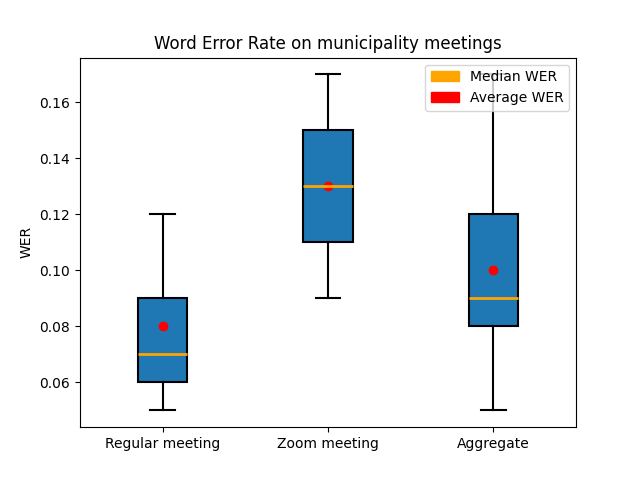
\includegraphics[width=0.85\textwidth]{images/whisperBench.png}
    \caption{Whisper ASR Performance on Municipality Meetings. This figure displays the Word Error Rate (WER) for Whisper across various meetings. The data, comprising 40 minutes of manually transcribed audio from seven different meetings spanning five years and three municipalities, was normalized to remove non-alphabetical characters and convert text to lowercase. Results show WER for regular meetings is consistent with Whisper benchmarks presented in \cite{radford2023robust}. Notably, WER is higher for Zoom meetings, likely due to varied audio quality from different devices and microphones used by participants.}
    \label{fig:whisperExperiment}
\end{figure}

as can be seen from figure \ref{fig:whisperExperiment}, the transcription WER in regular meetings is in line with what can be expected from the Whisper benchmarks presented in \cite{radford2023robust} (illustrated in figure \ref{fig:whisperwer}).
One interesting observation is the large difference between Zoom meetings and regular meetings. For a couple years during the nationwide COVID regulations, the municipality meetings took place online. During these meetings, every participant used their own device and microphone - a general lower audio quality - with large quality differences between different speakers probably contributing to lower transcription accuracy.

Another cause for error is when a speaker speaks quickly, without perfect articulation. 
An example of such a situation where Whisper gets confused, is visualized in figure \ref{fig:whisperResultWERVis1}. In this figure, green text represents a substitution, while red text represents a deletion. The snippet of text is taken from a 2019 Haarlem meeting, with code $622012$, starting at 01:47:10. Here, the speaker is not clearly understandable, resulting in a transcription not making the most sense. 
Luckily, these situations are not very common, as evidenced by the global WER given in figure \ref{fig:whisperExperiment}.

\begin{figure}[htbp]\caption{Visual example of Whisper ASR WER Analysis. This figure visualizes the WER for a snippet from a 2019 Haarlem meeting (code 622012) starting at 01:47:10. The Whisper generated reference transcription is compared with a manual transcription. Green text indicates substitutions, where a word in the hypothesis replaces a word in the reference. Red text indicates deletions, where words present in the reference are missing in the hypothesis. This example contains a fast, unclear speech, resulting in some transcription errors, with specific substitutions and deletions highlighted.}\label{fig:whisperResultWERVis1}
    \centering
\begin{Verbatim}[commandchars=\\\{\}]
reference: ... ben ik toch een beetje benieuwd naar de reactie van het college. 
En ik heb inderdaad ook het gevoel dat we vanavond toch al op het zuid gaan komen. 
Dus waarom zouden we dat nu nog geheim verklaaren? ...

hypothesis: ... ben ik toch een beetje benieuwd naar de reactie van het college. 
En ik heb inderdaad ook het gevoel er wordt vanavond gewoon een besluit genomen, 
dus waarom zouden we dat nu nog geheim verklaren? ...

WER delta: ... ben ik toch een beetje benieuwd naar de reactie van het college 
en ik heb inderdaad ook het gevoel \textcolor{green}{er} (dat) \textcolor{green}{wordt} (we) vanavond \textcolor{red}{toch al op} \textcolor{green}{gewoon} 
(het) \textcolor{green}{een} (zuid) \textcolor{green}{besluit} (gaan) \textcolor{green}{genomen} (komen) dus waarom zouden we dat nu nog 
geheim \textcolor{green}{verklaren} (verklaaren) ... 
\end{Verbatim}
\end{figure}

\subsection{Pyannote}\label{sec:pyanExp}
As described in section \ref{sec:pyannote}, speaker diarisation is scored based on the Diarisation Error Rate (DER). At the time of writing, pyannote.audio offers the best performing speaker diarisation, as shown in figure \ref{fig:pyanres}. 

To test how well pyannote performs on the municipality dataset, I manually annotated 30 random minutes of meetings, distributed over five different meetings, from four different municipalities over three years. I used audio tool Audacity \footnote{https://www.audacityteam.org/} to obtain millisecond-accurate timestamps. During manual diarisation, speakers were named arbitrarily. After diarisation, the manual speaker names were mapped to the speaker names given by pyannote to make sure the confusion rate metric can be performed.

One example of how a such a manual diarisation looks relative to a pyannote diarisation, can be seen in figure \ref{fig:manvspyan}. This snippet is taken from a Ridderkerk meeting in 2022, with code $938576$, starting at 00:41:10. As can be seen from the figure, the graph is mostly identical, ignoring some small starting- and ending points discrepancies. 
One thing that stands out however, is the addition of two very short speaking turns picked up by pyannote. The first occurrence of this happens around 2530 seconds, where speaker 17 allegedly starts talking. This turns out to be just some noise resulting from the Zoom. Another the other short speaking turn, occurring at around 2615 seconds, is just a noise made by a meeting member, not worthy of being classified as speech. 

\begin{figure}[htbp]
    \centering
    \begin{subfigure}{0.9\textwidth}
        \centering
        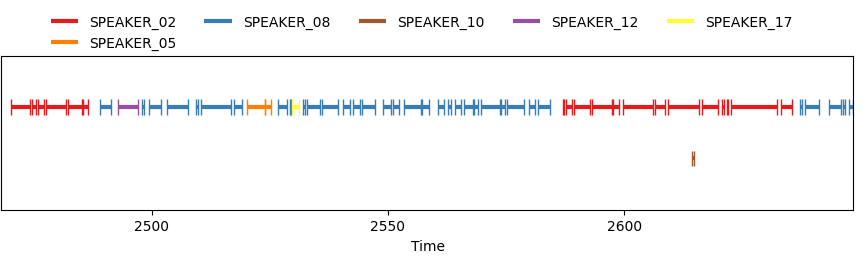
\includegraphics[width=\linewidth]{images/refDiar.png}
        \caption{pyannote diarisation}
        \label{fig:subfiga}
    \end{subfigure}
    \hfill
    \begin{subfigure}{0.9\textwidth}
        \centering
        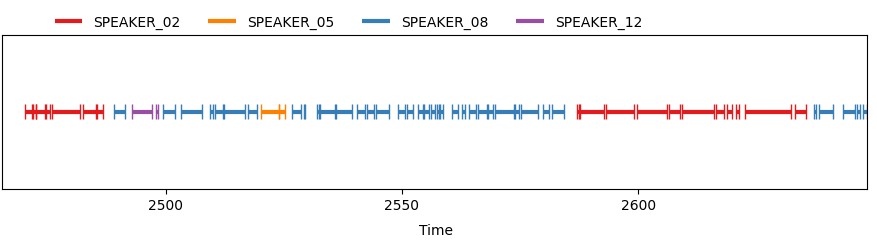
\includegraphics[width=\linewidth]{images/hypDiar.png}
        \caption{Manual diarisation}
        \label{fig:subfigb}
    \end{subfigure}
    \caption{Comparison of pyannote and Manual Diarisation for a Ridderkerk Meeting. This figure compares the pyannote.audio diarisation (a) with a manual diarisation (b) for a meeting in Ridderkerk, 2022 (code 938576), starting at 00:41:10. The graphs show overall agreement between the two methods, with minor, expectable discrepancies at the start and end points of speaking turns.}
    \label{fig:manvspyan}
\end{figure}

To address systemic differences in the idea when speech begins and ends, I performed two metrics. One with a 500-milliseconds collar, one with a 250-milliseconds collar, and one without a collar. 
A collar is a margin of time around each speaker's turn boundary. A 250 milliseconds collar would mean that the 125-milliseconds before and after each speaker change is excluded from evaluation.

\begin{figure}
    \centering
    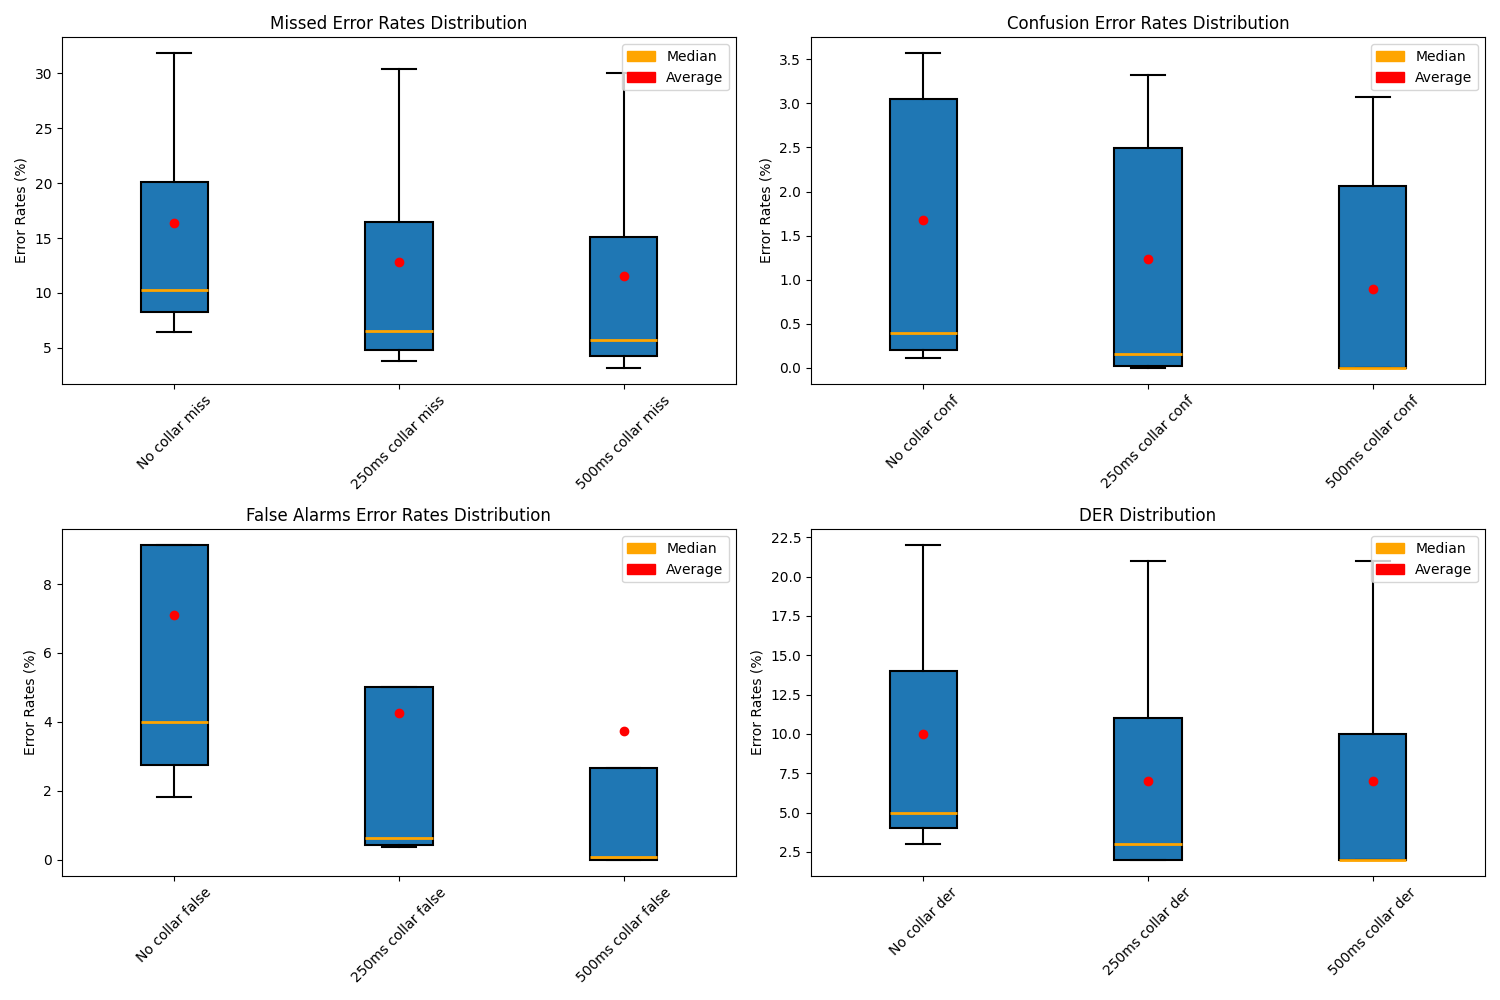
\includegraphics[width=0.98\textwidth]{images/error_rates_box_plots.png}
    \caption{Comparison of diarisation errors for pyannote.audio across different collar sizes (0 ms, 250 ms, 500 ms). Data were collected from over 30 minutes of annotated meetings, distributed over five different meetings from four municipalities spanning three years. The graph shows similar, if not slightly improved results from the official benchmarks in figure \ref{fig:pyanres}.}
    \label{fig:pyanExperiment}
\end{figure}

Comparing figure \ref{fig:pyanExperiment} to the benchmark results in figure \ref{fig:pyanres}, some interesting observations can be made. 
Firstly, the measured Confusion rate is significantly lower than the official benchmarks. Additionally, the average Miss- and False Alarm rates are roughly equivalent to those in the benchmark results. However, my application exhibits a few high outliers, predominantly originating from Zoom meetings. These outliers, as discussed in the previous section, are introduced by the same drawbacks associated with the online meeting environment.
Finally, the Diarisation Error Rate, combining all previous mentioned metrics, is again fairly similar to the official benchmarks, even including the Zoom outliers. 
For all evaluated metrics, the median values are either comparable to- or notably lower than those in the official benchmarks, indicating a strong general performance.
One potential reason as to why pyannote seems to perform better on these meetings, is the relatively simple structure of the meetings. There is not too much overlapping speech and speakers generally are speaking through good microphones.

\section{Agenda point segmentation}
Some meetings already had their agenda points uploaded and available in the archive. By using these pre-labeled agenda points as a ground truth, I tested the created topic segmentation script described in section \ref{sec:agendapoints}, thus answering research question 3.

I ran the segmentation script, represented in algorithm \ref{alg:topic}, on 10 different meetings over two years, using their provided agenda points as a ground truth. Next, I counted the number of missed agenda points and the number of false agenda points.

The disappointing results from figure \ref{fig:agendaSegmResults} indicate that the developed method of automatic topic segmentation in these types of government meetings is not sufficient yet. Based on the already available agenda points, a meeting has about nine agenda points on average. This information makes the results from figure \ref{fig:agendaSegmResults} even poorer. Although most true agenda points are labeled, a false positive rate of 5 topics per meeting, or more than 50\% on average, is just unacceptable.

Besides the uninspiring accuracy results, there are some other hurdles preventing topic segmentation from succeeding. One is the limited context window described in section \ref{sec:agendapoints}. 
Second is the sliding window approach used. Long meetings easily contain several thousand spoken sentences, all of which need to be fed to the LLM separately. Even with heavy optimization such as combining sentences, a single video can easily take multiple hours to process.

\begin{figure}[H]
    \centering
    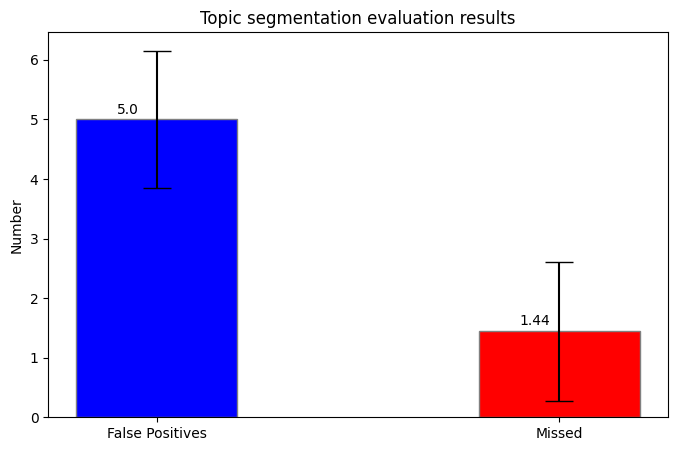
\includegraphics[width=0.85\textwidth]{images/topicSegmentation.png}
    \caption{Evaluation of automatic agenda point segmentation accuracy. The figure displays the performance of an automatic topic segmentation script tested on 10 different government meetings, distributed over two years. The evaluation, based on the number of missed and false agenda points compared to pre-labeled ground truth, reveals significant deficiencies: the segmentation method produced a false positive rate of more than 50\%, identifying approximately five incorrect topics per meeting. These results highlight the current limitations of the method, including the restricted context window and the inefficiency of the sliding window approach, which contributes to lengthy processing times.}
    \label{fig:agendaSegmResults}
\end{figure}

\section{Search engine}\label{sec:searchEngineExp}
In this section, the developed methods for research question 4 and 5 are evaluated. The implementation that is to be evaluated is directly embedded in the final search engine. Thus, this section indirectly also provides an evaluation to the implementation of the main research question, \textit{How can AI be utilized in order to increase information retrievability of large video archives, in particular of democratically elected councils}?
To do this, I gathered 13 participants and tasked them to find the answer to five questions using five different search methods.

\begin{enumerate}
    \item The contemporary way, scrolling through the video and using its agenda points;
    \item Using the vector search engine;
    \item Using the BM25 search engine;
    \item Using the hybrid search engine;
    \item Using the chat function.
\end{enumerate}

For each participant, the search methods were randomly mapped to a question. 
The participants first received a breakdown of the search engine, explaining how everything works. Then, they got some practice time to get familiar with the tools.
Then, when they felt comfortable with the search engine, the participants had three minutes to answer each question. In the scenario where a satisfactory answer is not found within the given time, the search is aborted and this is noted.

The questions were:
\begin{enumerate}
    \item What was the main reason given for the delay in the harmonising of outdoor sports?
    \item What are the expected advantages to the installation of the gardens surrounding underground trash containers?
    \item What is the difference between the first and second playgrounds?
    \item How late is the guest speaker awoken by the humming sound of nearby windmills?
    \item What is the goal of the proposal with regards the the 'gemeenschappelijke regeling van de bedrijfsvoeringspartner'?
\end{enumerate}

\begin{figure}
    \centering
    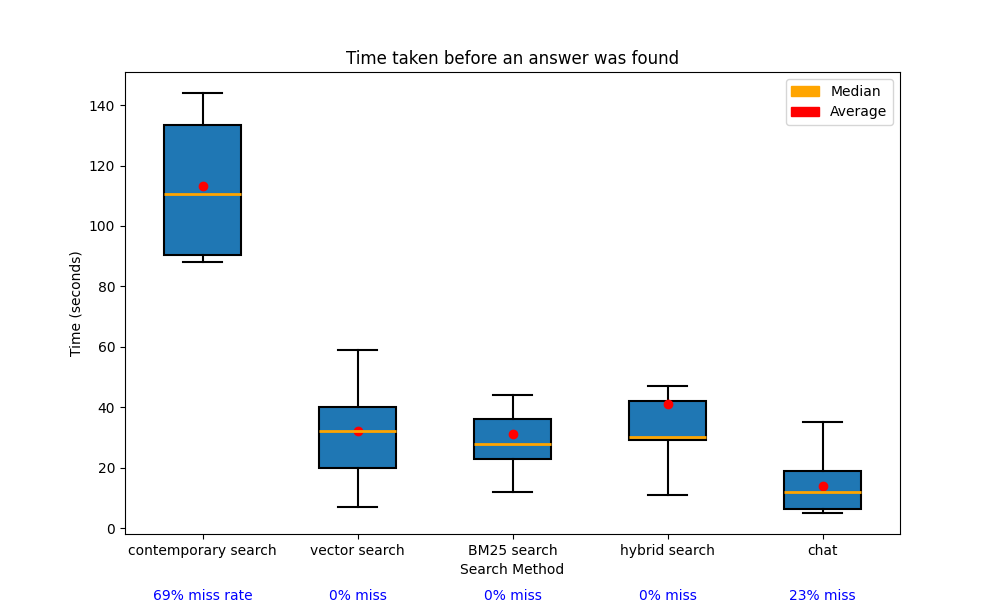
\includegraphics[width=0.98\textwidth]{images/search_methods_box_plot.png}
    \caption{omparison of Search Method Efficiency and Variability. The figure shows the average search times and variability for five search methods used by 13 participants to answer questions from video archives. Each participant was randomly assigned a search method for each question, and searches were conducted within a three-minute time limit. BM25 search was the most efficient among Weaviate methods, while the contemporary method of scrolling through video was the least efficient, failing to find an answer within the time limit 69\% of the time. Despite the chat function being the fastest on average, it struggled with validity, giving incorrect answers 23\% of the time.}
    \label{fig:engineResults}
\end{figure}

Figure \ref{fig:engineResults} shows the results of this experiment, disregarding the search attempts where an answer was not found in time. 
Observing these results, it can be concluded that the contemporary method of scrolling through the video is by far the least efficient. On top of the fact that the average search time is almost three times as slow as the second slowest method, in 69\% of the cases, a valid answer was not found within the given three minutes.

The three Weaviate search methods all performed roughly equal, with BM25 taking the lead. As can be seen, vector search brought a higher degree of variability with it. Despite this variability, the interquartile range is not remarkably high compared to the other Weaviate search methods. 

On the surface the chat functionality seems to work the quickest. However, this could have something to do with the specific questions asked. For about 23\% of the participants, the chat functionality could not give a valid answer. This is because if the answer to the questions is not among the top results returned by Weaviate, the LLM will not be capable of answering the question. In some cases, the LLM even hallucinated an answer, thinking it was correct despite this not being the case. 
In the prompt the LLM is tasked to answer that it does not know something if the information is not in the provided context. Sometimes, this instruction is not properly followed and the LLM will make up an answer.
Unfortunately, it is not easily detectable when an answer is a hallucination or true. Thus, one should not rely without second thought on answers given by the chat bot. When receiving a response, the answer should always be verified.


\chapter{Conclusion}
Looking back at the main research question \textit{how can AI be utilized in order to increase information retrievability of large video archives, in particular of democratically elected councils}? It can be concluded from figure \ref{fig:engineResults} that a strong and user friendly system of information retrievability has indeed been developed, as indicated by the significantly quicker retrieval times. 

This has been achieved by making use of a custom written Whisper ASR and pyannote.audio speaker diarisation pipeline. In this pipeline, videos are transcribed and diarised, after which they are embedded and inserted in a Weaviate vector database. Both video analysis tool implementations and the Weaviate are measured to perform either on par with- or better than the current state-of-the-art benchmark evaluations, answering the research question \textit{what state-of-the-art video- and audio analysis tools can be used to improve searchability of the meetings, and how accurate are these in the given circumstances}? and \textit{what state-of-the-art information retrieval techniques can be leveraged to develop an efficient video information retrieval system}?.

The research question topic segmentation research question, \textit{how accurately can such a video be segmented into the meaningfully different parts which are discussed}? did not receive an answer as positive as the previous research questions. It turned out that several contemporary complications, namely context window and compute power, hindered the development of creating an accurate topic segmentation system usable in governmental meeting archives.

Finally, a chat bot system with access to the Weaviate database allows the user to ask questions regarding specific meetings in a conversational style. As shown in figure \ref{fig:engineResults}, this chat bot scores significantly better than the contemporary search method and slightly better than the three other implemented search methods, indicating that the research question \textit{how well can the developed search system be integrated with a large language model, creating a helpful chat bot capable of answering questions and providing complementary information when needed}? can be positively answered, with the caveat that the chat bot will sometimes hallucinate if it can not find an answer. It is hard to know exactly when responses are hallucinations, meaning manual verification is always necessary when receiving an answer from the chat bot.

% Ik denk dat ik hier nog iets wil over een toekomstig onderzoek waar nog meer naar gekeken kan worden? IDK

% Ook een afbeelding toevoegen van de verschillende gains in zoom meetings en geen zoom meetings die dat aantoont??


\printbibliography

\end{document}
